%%%%%%%%%%%%%%%%%%%%%%%%%%%%%%%%%%%%%%%%%%%%%%%%%%%%%%%%%%%%%%
\documentclass[a4paper]{article}
\usepackage[margin=2.5cm, top=2cm, left=3cm]{geometry}
\usepackage[T1]{fontenc}
\usepackage{mathptmx}
\usepackage{blindtext}
\usepackage{enumitem}
\usepackage{setspace}
\usepackage{algorithm}
\usepackage{algorithmic}
\usepackage[linesnumbered,ruled,vlined]{algorithm2e}
\usepackage{booktabs}
\usepackage[vietnamese, english]{babel}
\usepackage{float}
\usepackage{amsmath,amssymb,amsfonts}
\usepackage{graphicx}
\usepackage{minted}
\usepackage{xcolor}
\usepackage{scrextend}
\usepackage{array}
\definecolor{LightGray}{gray}{0.9}
%\usepackage{background}
\usepackage{xcolor}
\usepackage{minted}
\usepackage{hyperref}       % hyperlinks
\hypersetup{
    filecolor=magenta,
    urlcolor=cyan,
    citecolor=blue,
    pdftitle={ỨNG DỤNG GIẢI THUẬT DI TRUYỀN GIẢI BÀI TOÁN KNAPSACK},
    pdfpagemode=FullScreen,
    }
\usepackage{url}            % simple URL typesetting
\usepackage[nameinlink, capitalise, noabbrev]{cleveref}
\usepackage{booktabs}       % professional-quality tables
\usepackage{amsfonts}       % blackboard math symbols
\usepackage{nicefrac}       % compact symbols for 1/2, etc.
\usepackage{microtype}      % microtypography
\usepackage{natbib}
\usepackage{titlesec}
\usepackage{tikz}
\usetikzlibrary{calc}
\usepackage{pgfplots}
\usepackage{color}
\pagestyle{plain}
\usepackage{fancyhdr}
\fancyhf{}
\cfoot{\thepage}
\titleformat*{\section}{\fontsize{13pt}{13}\bfseries}
\titleformat*{\subsection}{\fontsize{13pt}{13}\bfseries}
\titleformat*{\subsubsection}{\fontsize{13pt}{13}\bfseries}
%%%%%%%%%%%%%%%%%%%%%%%%%%%%%%%%%%%%%%%%%%%%%%%%%%%%%%%%%%%%%%
\begin{document}

%%%%%%%%%%%%%%%%%%%%%%%%%%%%%%%%%%%%%%%%%%%%%%%%%%%%%%%%%%%%%%
\fontsize{13pt}{15pt}\selectfont
\setlength{\parindent}{0cm}
\setlength{\parskip}{1.5ex}
\setlength{\baselineskip}{1.5\baselineskip}
%%%%%%%%%%%%%%%%%%%%%%%%%%%%%%%%%%%%%%%%%%%%%%%%%%%%%%%%%%%%%%
\begin{otherlanguage*}{vietnamese}
\begin{titlepage}

\begin{tikzpicture}[remember picture, overlay]
  \draw[line width = 2pt] ($(current page.north west) + (0.5in,-0.5in)$) rectangle ($(current page.south east) + (-0.5in,0.5in)$);
\end{tikzpicture}
 
\begin{center}

% Upper part of the page
\Large BỘ GIÁO DỤC VÀ ĐÀO TẠO\\[7pt]
\textbf{\Large ĐẠI HỌC KINH TẾ THÀNH PHỐ HỒ CHÍ MINH}\\[1cm]
\begin{figure}[!h]
    \centering
    
\includegraphics[width=4cm]{ueh.png}
\end{figure}

\vspace{1cm}

\Large\textbf{ĐỒ ÁN MÔN HỌC}\\[0.5cm]
\Large{TRÍ TUỆ NHÂN TẠO}\\ [1cm]
\Large\textbf{ỨNG DỤNG GIẢI THUẬT DI TRUYỀN GIẢI BÀI TOÁN KNAPSACK}
\end{center}
\vspace{1cm}

\textbf{{Nhóm sinh viên thực hiện:}}

\begin{tabbing}
\hspace{8cm}\=\hspace{6cm}\=\hspace{6cm} \kill
{\textbf{Họ và tên}}\>{\textbf{MSSV}}\>{\textbf{Lớp}}\\
Nguyễn Quốc Việt \> 31211027687 \> DS001\\
Vũ Nguyễn Thảo Vi \> 31211027686 \> DS001\\
Đinh Trọng Hữu \> 31211027643 \> DS001\\
Nguyễn Quang Nhật \> 31211027658 \> DS002\\
Phan Đình Nhân \> 31211027657 \> DS001\\
\end{tabbing}

\begin{center}

\textbf{Khoá:} K47

\textbf{Chuyên ngành: } Khoa học dữ liệu

\end{center}

\begin{center}
\large \textbf{GVHD:} TS. Đặng Ngọc Hoàng Thành\\
\end{center}

% Bottom of the page
\vfill
\begin{center}
\vspace{0.5cm}
\large \textbf{TP. Hồ Chí Minh, {\selectlanguage{vietnamese}\today}}
\end{center}

\end{titlepage}

%%%%%%%%%%%%%%%%%%%%%%%%%%%%%%%%%%%%%%%%%%%%%%%%%%%%%%%%%%%%%%

\tableofcontents
\pagebreak

\section{Tổng Quan}

\subsection{Giới thiệu về vấn đề Knapsack}
Knapsack (túi đồ) là một bài toán tối ưu hóa trong khoa học máy tính, trong đó một túi có giới hạn dung lượng và một tập hợp các đồ vật, mỗi đồ vật có giá trị và khối lượng khác nhau. Mục tiêu của bài toán là đưa các đồ vật vào túi sao cho tổng giá trị của các đồ vật này là lớn nhất, và tổng khối lượng của các đồ vật không vượt quá dung lượng giới hạn của túi.

Bài toán knapsack có thể được biểu diễn bằng một cặp $(W, v)$, trong đó $w$ là một mảng chứa khối lượng của từng đồ vật và $v$ là một mảng chứa giá tiền của từng đồ vật. Với một túi có dung lượng tối đa $W$, mục tiêu của bài toán là chọn một tập con của các đồ vật sao cho tổng khối lượng của các đồ vật này không vượt quá $W$ và tổng giá trị của các đồ vật này là lớn nhất.

Bài toán knapsack là một bài toán quen thuộc trong lĩnh vực tối ưu hóa và có ứng dụng trong nhiều lĩnh vực khác nhau, chẳng hạn như quản lý kho, tối ưu hóa chi phí sản xuất, tối ưu hóa đầu tư và tài chính, và các vấn đề liên quan đến vận chuyển và đóng gói.

\subsection{Phát biểu bài toán}

Bài toán Knapsack là bài toán tối ưu tổ hợp (combinatorial optimization). Cho trước $n$ vật, mỗi vật với cân nặng $w_{i}$ và giá trị $v_{i}$ và sức chứa tối đa của ba lô là $W$, mục tiêu của bài toán là tìm ra một tập hợp các vật để tối đa hoá giá trị của các vật phẩm trong ba lô sao cho các vật phẩm đã chọn không được vượt quá sức chưa tối đa của ba lô.

Ta phát biểu bài toán như sau:

\begin{itemize}
\item Cho $n$ là số vật phẩm
\item $w_{i}$ là cân nặng của vật thứ $i$ ($1 \leq i  \leq n$)
\item $v_{i}$ là giá trị của vật thứ $i$ ($1 \leq i  \leq n$)
\item $W$ là khả năng chứa tối đa của ba lô.
\item $x_{i}$ là biến nhị phân biểu diễn một vật có được chọn hay không. Nếu $x_{i} =1$ thì vật được chọn và ngược lại, nếu $x_{i} = 0$ thì vật không được chọn.
\end{itemize}

Khi đó, bài toán Knapsack có thể được biểu diễn dưới dạng một bài toán quy hoạch tuyến tính như sau:

\begin{center}
    
$max \sum_{i=1}^{n} v_{i}x_{i}$ 

với $\sum_{i=1}^{n} w_{i}x_{i} \leq W$ và $x_{i} \in \{0,1\}$, $1 \leq i \leq n$

\end{center}


\subsection{Một Số Hướng Tiếp Cận Giải Quyết Bài Toán}
Có nhiều hướng tiếp cận để giải quyết bài toán Knapsack, trong đó các phương pháp sau đây là phổ biến nhất:

\begin{enumerate}[leftmargin=7pt]
    \item \textbf{Brute-force:} Cách tiếp cận đơn giản nhất là liệt kê tất cả các tập con của tập hợp đồ vật, kiểm tra xem tập con nào có tổng trọng lượng không vượt quá giới hạn trọng lượng của túi và có giá trị lớn nhất.
    Brute-force là cách tiếp cận đơn giản nhất để giải quyết bài toán knapsack, tuy nhiên, nó không hiệu quả khi số lượng đồ vật và giới hạn trọng lượng túi là lớn. Các bước thực hiện của brute-force như sau:
    
\begin{itemize}[leftmargin=7pt]
\item Liệt kê tất cả các tập con của tập hợp đồ vật.
\item Kiểm tra xem tập con nào có tổng trọng lượng không vượt quá giới hạn trọng lượng của túi.
\item Tìm tập con có giá trị lớn nhất trong các tập con hợp lệ.
Độ phức tạp tính toán của brute-force là $O(2^n)$, với n là số lượng đồ vật. Vì vậy, với n lớn, brute-force không thể được sử dụng để giải quyết bài toán knapsack.
\end{itemize}
\item \textbf{Greedy algorithms} là phương pháp tham lam để giải quyết bài toán knapsack, tức là chọn các đồ vật dựa trên một tiêu chí tối ưu hóa nhất định. Các bước thực hiện của greedy algorithms như sau:

\begin{itemize}[leftmargin=7pt]
\item Sắp xếp các đồ vật theo thứ tự giá trị giảm dần hoặc trọng lượng tăng dần.
\item Chọn đồ vật đầu tiên và thêm vào túi, tiếp tục chọn đồ vật thứ hai, thứ ba, cho đến khi đạt giới hạn trọng lượng của túi hoặc hết các đồ vật.    
\end{itemize}

Tuy nhiên, giải pháp tham lam không đảm bảo sẽ tìm được lời giải tối ưu cho mọi trường hợp. Ví dụ, nếu ta có các đồ vật với giá trị lớn nhưng trọng lượng rất nặng, việc chọn đồ vật theo thứ tự giá trị giảm dần sẽ dẫn đến việc bỏ lỡ một số đồ vật có trọng lượng nhỏ hơn nhưng giá trị cao hơn.

Vì vậy, greedy algorithms có thể được sử dụng để giải quyết bài toán knapsack với các giới hạn thời gian và bộ nhớ hạn chế, nhưng không đảm bảo tìm ra giải pháp tối ưu.

\section{Giải thuật di truyền} \label{sec:ga}
\subsection{Giới thiệu về Giải thuật di truyền}

Giải thuật di truyền (GA) là một phương pháp tối ưu hóa tự động bằng cách sử dụng các khái niệm và kỹ thuật liên quan đến di truyền học. Thuật toán này lấy cảm hứng từ quá trình tiến hóa tự nhiên vào việc tối ưu hóa các hàm mục tiêu bằng cách sử dụng các phép toán và quy luật trong sinh sản và tiến hóa của các cá thể. Cụ thể, trong tự nhiên các loài sinh vật tiến hóa thông qua các quá trình di truyền gen từ thế hệ này sang thế hệ khác và chọn lọc tự nhiên, trong đó các cá thể mạnh mẽ và phù hợp với môi trường sống được lựa chọn để tiếp tục phát triển và sinh sản.

Tương tự, giải thuật di truyền sử dụng quy trình tương tự để tìm kiếm giải pháp tối ưu. Các cá thể trong quần thể được đại diện bởi các giải pháp khác nhau và được đánh giá dựa trên một hàm mục tiêu. Các cá thể tốt nhất được chọn để lai ghép và đột biến tạo ra các cá thể mới, và quá trình này được lặp lại để tìm kiếm giải pháp tối ưu.

Giải thuật di truyền có khả năng tìm được các giải pháp tối ưu cho các không gian tìm kiếm phức tạp và không liên tục. Điều này là do giải thuật di truyền không yêu cầu các giải pháp phải có tính liên tục hay đạo hàm, và có khả năng tìm kiếm toàn cục thông qua việc duy trì một quần thể đa dạng.

Ngoài ra, giải thuật di truyền cũng có khả năng tìm kiếm các giải pháp tối ưu đối với các bài toán tối ưu hóa đa mục tiêu, trong đó có nhiều hàm mục tiêu cần được tối ưu hóa đồng thời.

Việc tìm giải pháp tối ưu với giải thuật di truyền phụ thuộc vào nhiều yếu tố như cấu hình tham số của giải thuật, kích thước quần thể, hàm đánh giá và phép lai ghép, đột biến được sử dụng. Nếu không lựa chọn cẩn thận các tham số và các phép toán, GA có thể không thể tìm được giải pháp tối ưu cho một số bài toán. Giải thuật di truyền được ứng dụng rộng rãi trong các bài toán tối ưu hóa, sắp xếp thời khoá biểu, thiết kế mạch điện tử, robot học, phân tích dữ liệu, và nhiều lĩnh vực khác. Đặc biệt, giải thuật di truyền còn là một công cụ hữu ích cho các nhà nghiên cứu trong việc giải quyết các bài toán phức tạp, không thể được biểu diễn dưới dạng công thức toán học và do vậy khó có thể giải quyết bằng các phương pháp truyền thống.

Các bước trong giải thuật di truyền có thể được biểu diễn như sau:

\begin{figure}[!h]
    \centering
    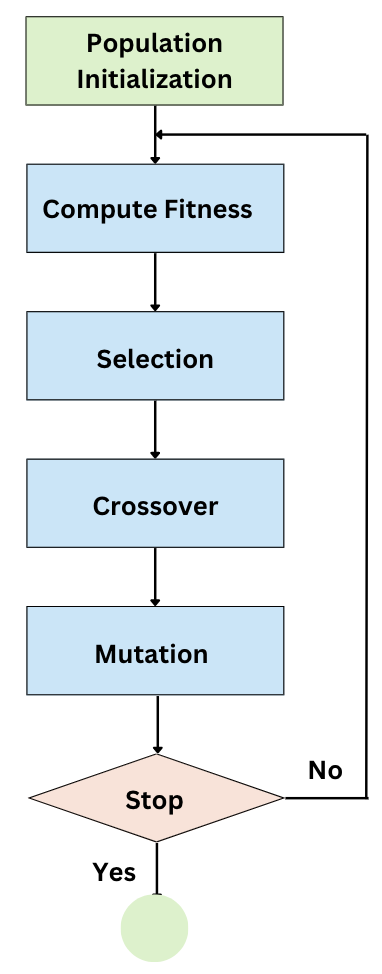
\includegraphics[width=4.5cm]{ga.png}
    \caption{Lưu đồ giải thuật di truyền}
    \label{fig:ga}
\end{figure}

Các bước chính trong giải thuật di truyền bao gồm:

\begin{enumerate}[leftmargin=7pt]
\item \textbf{Khởi tạo quần thể (Population Initialization):} Tạo ra một tập hợp các cá thể ngẫu nhiên để đại diện cho các giải pháp có thể trong không gian tìm kiếm.

\item \textbf{Tính hàm Fitness:} Đánh giá mức độ thích nghi của từng cá thể với bài toán.

\item \textbf{Lựa chọn (Selection):} Chọn ra một số lượng cá thể tốt nhất để tiếp tục phát triển trong thế hệ kế tiếp. Các phương pháp lựa chọn có thể là chọn lọc tự nhiên, chọn lọc xếp hạng, hay chọn lọc theo roulette wheel.

\item \textbf{Lai ghép (Crossover):} Sử dụng các toán tử lai ghép để tạo ra các cá thể mới từ các cá thể đã chọn trong bước trước đó. Các phương pháp lai ghép bao gồm lai một điểm, lai nhiều điểm, lai đồng nhất, và lai khác loại.

\item \textbf{Đột biến (Mutation):} Áp dụng các toán tử đột biến để tạo ra sự đa dạng cho quần thể bằng cách thay đổi các gene của các cá thể. Các phương pháp đột biến bao gồm đột biến đơn giản, đột biến đảo ngược, và đột biến ngẫu nhiên.

\item \textbf{Đánh giá cá thể (Evaluation):} Sử dụng một hàm mục tiêu để đánh giá hiệu suất của mỗi cá thể trong quần thể.

\item \textbf{Kiểm tra điều kiện dừng:} Kiểm tra xem giải thuật đã đạt được kết quả tối ưu hay chưa. Nếu chưa, quay lại bước 2. Nếu đã đạt được kết quả tối ưu, kết thúc quá trình.

\end{enumerate}

Pseudocode của giải thuật di truyền có thể được biểu diễn như sau:

\begin{algorithm}[H]
GA(Fitness,$\theta,n,r_{co},r_{mu}$)

\KwData{

Fitness: A function that produces the score (fitness) given a hypothesis

$\theta$: The desired fitness value (i.e., a threshold specifying the termination condition)

$n$:  The number of hypotheses in the population

$r_{co}$:  The percentage of the population influenced by the crossover operator at each step

$r_{mu}$:  The percentage of the population influenced by the mutation operator at each step
}
\KwResult{Optimal solution}
Initialize the population: $H$ Randomly generate $n$ hypotheses;

Evaluate the initial population. For each $h \in H$ compute Fitness(h);

\While{$max_{\{h \in H\}}Fitness(h) < \theta$}{
$H^{next} $;

\textbf{Reproduction}

Probabilistically select $(1-r_{co})n$ hypotheses of H to add to $H^{next}$;

The probability of selecting hypothesis $h_{i}$ from H is $P(h_{i}) = \frac{Fitness(h_{i})}{\sum_{j=1}^{n}Fitness(h_{j})}$;

\textbf{Crossover}

Probabilistically select  $(r_{co}.n/2)$ pairs of hypotheses from H, according to the probability computation $P(h)$ given above.

For each pair  $(h_{i}, h_{j})$, produce two offspring (i.e., children) by applying the crossover operator. Then, add all the offspring to $H^{next}$.

\textbf{Mutation}

Select  $(r_{mu}.n)$  hypotheses of $H_{next}$, with uniform probability.

For each selected hypothesis, invert one randomly chosen bit (i.e., 0 to 1, or 1 to 0) in the hypothesis’s representation or 1 to 0)in the hypothesis's representation.

Producing the next generation:  $H \leftarrow H^{next}$

Evaluate the new population. For each $h \in H$:  compute Fitness($h$)

}
\Return $argmax_{h \in H}Fitness(h)$;
\caption{Genetic Algorithm}
\end{algorithm}

\subsection{Ứng dụng Giải thuật di truyền cho bài toán Knapsack}

Bài toán Knapsack có thể được giải quyết bằng Giải thuật di truyền (Genetic Algorithm - GA) bằng cách sử dụng chuỗi nhị phân để biểu diễn mỗi lời giải. Cụ thể, mỗi nhiễm sắc thể trong quần thể đại diện cho một lời giải, với mỗi gene trong chuỗi nhị phân tương ứng với một vật có được chọn hay không trong túi.

\begin{itemize}[leftmargin=7pt]
\item 
Hàm generate\_random\_value() trả về một giá trị ngẫu nhiên thuộc tập {0, 1}. Đây là hàm được sử dụng để khởi tạo các gene (gen) trong chuỗi nhị phân của nhiễm sắc thể (chromosome) trong bài toán Knapsack.

Hàm này sử dụng hàm randint() từ thư viện random để sinh ngẫu nhiên một số nguyên trong khoảng từ 0 đến 1 (bao gồm cả 0 và 1). Nếu số sinh ra là 0, tức là vật không được chọn, và nếu số sinh ra là 1, tức là vật được chọn.

\begin{minted}
[frame=lines,framesep=2mm,baselinestretch=1.2,fontsize=\small,linenos]{python}
def generate_random_value():  
    return random.randint(0, 1) 
\end{minted}

\item 
Hàm create\_individual() được sử dụng để tạo ra một cá thể (chromosome) mới cho quần thể. Mỗi cá thể được biểu diễn bằng một chuỗi nhị phân có độ dài bằng số lượng vật trong bài toán Knapsack.

Hàm này sử dụng hàm generate\_random\_value() để tạo ra các gene trong chuỗi nhị phân của nhiễm sắc thể. Nó sử dụng một vòng lặp for để tạo ra một list chứa n giá trị ngẫu nhiên thuộc tập {0, 1} sử dụng hàm generate\_random\_value(). Cuối cùng, nó trả về list này như một cá thể mới.

\begin{minted}
[frame=lines,framesep=2mm,baselinestretch=1.2,fontsize=\small,linenos]{python}
def create_individual():
    return [generate_random_value() for _ in range(n)]
\end{minted}

\item 
Hàm compute\_fitness trên là một hàm tính toán độ thích nghi của một cá thể (chromosome) trong bài toán knapsack.

Cụ thể, hàm này nhận đầu vào là một cá thể (chromosome) và các thông số của bài toán knapsack gồm giá trị của các đối tượng (values), trọng lượng của các đối tượng (weights) và giới hạn trọng lượng của túi (max\_weight).

Trong hàm này, trọng lượng của cá thể được tính bằng cách nhân trọng lượng của mỗi đối tượng với số lượng đối tượng tương ứng được chọn trong cá thể, và giá trị của cá thể được tính bằng cách nhân giá trị của mỗi đối tượng với số lượng đối tượng tương ứng được chọn trong cá thể.

Nếu trọng lượng của cá thể vượt quá giới hạn trọng lượng của túi (max\_weight), hàm trả về giá trị là 0, ngược lại hàm trả về giá trị của cá thể đó.

\begin{minted}
[frame=lines,framesep=2mm,baselinestretch=1.2,fontsize=\small,linenos]{python}
def compute_fitness(chromosome, values, weights, max_weight):
    value = sum([chromosome[i] * values[i] for i in range(len(chromosome))])
    weight = sum([chromosome[i] * weights[i] for i in range(len(chromosome))])
    if weight > max_weight:
        return 0
    else:
        return value
\end{minted}

\item 
Hàm compute\_weight trên là một hàm tính toán trọng lượng của một cá thể (chromosome) trong bài toán knapsack.

Cụ thể, hàm này nhận đầu vào là một cá thể (chromosome) và thông số của bài toán knapsack là trọng lượng của các đối tượng (weights).

Trong hàm này, trọng lượng của cá thể được tính bằng cách nhân trọng lượng của mỗi đối tượng với số lượng đối tượng tương ứng được chọn trong cá thể, và tổng hợp lại.

Hàm compute\_weight này thường được sử dụng trong các giải thuật di truyền để tính toán trọng lượng của các cá thể trong quần thể và kiểm tra xem các cá thể có vượt quá giới hạn trọng lượng của túi (max\_weight) không.

\begin{minted}
[frame=lines,framesep=2mm,baselinestretch=1.2,fontsize=\small,linenos]{python}
def compute_weight(chromosome, weights):
    return sum([chromosome[i] * weights[i] for i in range(len(chromosome))])
\end{minted}

\item 
Hàm selection trên là một hàm thực hiện phép chọn lọc cá thể trong quần thể dựa trên độ thích nghi của các cá thể.

Cụ thể, hàm này nhận đầu vào là một danh sách các cá thể (population) và một danh sách các điểm đánh giá độ thích nghi tương ứng với mỗi cá thể (fitness\_scores).

Trong hàm này, ta lần lượt chọn ra các cá thể có độ thích nghi cao nhất trong quần thể, bằng cách tìm chỉ số của cá thể có giá trị điểm đánh giá cao nhất trong danh sách fitness\_scores, sau đó thêm cá thể đó vào danh sách selected\_chromosomes và đặt giá trị của điểm đánh giá tương ứng với cá thể đó trong fitness\_scores bằng 0 để không chọn lại cá thể này lần nữa.

Việc lặp lại trên sẽ được thực hiện cho đến khi danh sách selected\_chromosomes chứa đủ nửa số lượng các cá thể trong quần thể (do mỗi lần lặp lấy ra được 2 cá thể).

Sau khi hoàn thành việc chọn lọc, hàm trả về danh sách các cá thể đã được chọn (selected\_chromosomes).

Hàm selection này thường được sử dụng trong các giải thuật di truyền để tạo ra thế hệ tiếp theo của quần thể bằng cách sử dụng các cá thể được chọn để tiến hành lai ghép (crossover) và đột biến (mutation).

\begin{minted}
[frame=lines,framesep=2mm,baselinestretch=1.2,fontsize=\small,linenos]{python}
def selection(sorted_population):
    index1 = random.randint(0, m-1)
    while True:
        index2 = random.randint(0, m-1)
        if index2 != index1:
            break
    individual = sorted_population[index1]
    if index1 < index2:
        individual = sorted_population[index2]
    return individual
\end{minted}

\item 
Hàm crossover trên là một hàm thực hiện phép lai ghép giữa hai cá thể cha mẹ để tạo ra hai cá thể con mới.

Cụ thể, hàm này nhận đầu vào là hai cá thể cha mẹ (parent1, parent2) có cùng độ dài.

Trong hàm này, ta tạo ra một chỉ số ngẫu nhiên split\_index để phân chia hai cá thể cha mẹ thành hai phần. Điểm phân chia này được chọn ngẫu nhiên trong khoảng từ 1 đến độ dài của một trong hai cá thể cha mẹ (ở đây ta chọn độ dài của parent1).

Sau khi đã chọn được điểm phân chia, ta tạo ra hai cá thể con mới bằng cách ghép phần đầu của parent1 với phần sau của parent2 để tạo ra con thứ nhất, và ghép phần đầu của parent2 với phần sau của parent1 để tạo ra con thứ hai.

Cuối cùng, hàm trả về hai cá thể con mới (child1, child2) đã được tạo ra từ phép lai ghép giữa hai cá thể cha mẹ.

Hàm crossover này thường được sử dụng trong các giải thuật di truyền để tạo ra thế hệ tiếp theo của quần thể bằng cách sử dụng các cá thể được chọn từ hàm selection và áp dụng phép lai ghép này để tạo ra các cá thể con mới.

\begin{minted}
[frame=lines,framesep=2mm,baselinestretch=1.2,fontsize=\small,linenos]{python}
def crossover(parent1, parent2):
    split_index = random.randint(1, len(parent1)-1)
    child1 = parent1[:split_index] + parent2[split_index:]
    child2 = parent2[:split_index] + parent1[split_index:]
    return child1, child2
\end{minted}

\item 
Hàm mutate trên là một hàm thực hiện phép đột biến trên một cá thể.

Cụ thể, hàm này nhận đầu vào là một cá thể chromosome và một tỉ lệ đột biến mutation\_rate.

Trong hàm này, ta duyệt qua từng phần tử của chromosome và với mỗi phần tử đó, ta sẽ chọn ngẫu nhiên một số trong khoảng từ 0 đến 1. Nếu số này nhỏ hơn mutation\_rate, ta sẽ thực hiện đột biến bằng cách đảo bit của phần tử đó (nghĩa là nếu phần tử đó ban đầu bằng 0, ta sẽ đổi thành 1, và ngược lại).

Sau khi đã duyệt qua tất cả các phần tử của chromosome, hàm trả về cá thể chromosome đã được đột biến.

Hàm mutate này thường được sử dụng trong các giải thuật di truyền để giúp tăng độ đa dạng của quần thể, từ đó giúp giải thuật tìm được các giải pháp tốt hơn cho bài toán.

\begin{minted}
[frame=lines,framesep=2mm,baselinestretch=1.2,fontsize=\small,linenos]{python}
def mutate(individual, mutation_rate = 0.05):
    individual_new = individual.copy()
    if random.random() < mutation_rate:
        index = random.randint(0, n-1)
        individual_new[index] = generate_random_value()
    return individual_new
\end{minted}

\item 
Hàm genetic\_algorithm là hàm thực hiện giải thuật di truyền để giải bài toán knapsack.

Cụ thể, hàm này nhận đầu vào là số lượng items n\_items, một danh sách giá trị values tương ứng với các items, một danh sách trọng lượng weights tương ứng với các items, trọng lượng tối đa max\_weight của cái túi, kích thước quần thể population\_size, số đời tối đa generations, và tỉ lệ đột biến mutation\_rate.

Trong hàm này, ta bắt đầu bằng việc tạo ra một quần thể population bằng cách sử dụng hàm create\_individual để tạo ra các cá thể đầu tiên.

Sau đó, ta tiến hành lặp lại quá trình di truyền trong số đời generations cho trước. Trong mỗi đời, ta tính toán độ thích nghi (fitness) của từng cá thể trong quần thể, và chọn ra top các cá thể để sinh sản tiếp theo bằng hàm selection. Sau đó, ta tiến hành lai ghép (crossover) các cá thể được chọn để tạo ra đời con mới, và thực hiện phép đột biến (mutation) trên các đời con này bằng hàm mutate. Cuối cùng, ta thay thế quần thể cũ bằng đời con mới.

Sau khi đã hoàn thành số đời generations, ta tìm ra cá thể trong quần thể có độ thích nghi (fitness) cao nhất, và từ đó tìm ra các item được chọn và giá trị và trọng lượng tương ứng của chúng.

Hàm genetic\_algorithm sử dụng giải thuật di truyền để giải quyết bài toán knapsack, và thường được sử dụng trong các bài toán tối ưu hóa, tìm kiếm và khai thác dữ liệu.

\begin{minted}[frame=lines,framesep=2mm,baselinestretch=1.2,fontsize=\small,linenos]{python}
def genetic_algorithm(n_items, values, weights, max_weight,
population_size=100, generations=100, mutation_rate=0.001):
    # create the initial population
    population = [create_individual(n_items) for i in range(population_size)]
    # run the genetic algorithm for the specified number of generations
    for generation in range(generations):
    # calculate the fitness of each chromosome in the population
        fitness_scores = [compute_fitness(chromosome, values, weights, max_weight) 
        for chromosome in population]

    # select the top chromosomes for reproduction
    selected_chromosomes = selection(population, fitness_scores)

    # crossover the selected chromosomes to create new offspring
    offspring = []
    for i in range(population_size // 2):
        parent1 = selected_chromosomes[random.randint(0, len(selected_chromosomes)-1)]
        parent2 = selected_chromosomes[random.randint(0, len(selected_chromosomes)-1)]
        child1, child2 = crossover(parent1, parent2)
        offspring.extend([child1, child2])

    # mutate the offspring
    for i in range(len(offspring)):
        offspring[i] = mutate(offspring[i], mutation_rate)

    # replace the old population with the new offspring
    population = offspring

# find the chromosome with the highest fitness score
best_chromosome = population[0]
best_fitness_score = compute_fitness(best_chromosome, values, weights, max_weight)
for chromosome in population:
    fitness_score = compute_fitness(chromosome, values, weights, max_weight)
    if fitness_score > best_fitness_score:
        best_chromosome = chromosome
        best_fitness_score = fitness_score

# return the solution
selected_items = [i+1 for i in range(n_items) if best_chromosome[i] == 1]
solution = {
    'items': selected_items,
    'value': best_fitness_score,
    'weight': compute_weight(best_chromosome, weights)
}
return solution
\end{minted}

\end{itemize}

\subsection{Độ phức tạp của Giải thuật di truyền}

Độ phức tạp của giải thuật di truyền phụ thuộc vào các yếu tố như kích thước của bài toán, kích thước của quần thể, tần suất đột biến và lai ghép, và hàm đánh giá, cụ thể:

\begin{itemize}[leftmargin=7pt]
\item Kích thước của bài toán ảnh hưởng đến số lượng cá thể cần để tiến hóa và số lượng thế hệ cần thiết để tìm ra giải pháp tối ưu. Kích thước của quần thể ảnh hưởng đến thời gian chạy của giải thuật và độ chính xác của kết quả. Quần thể càng lớn thì giải thuật càng có khả năng tìm ra giải pháp tối ưu, nhưng cũng tốn nhiều thời gian để thực thi.

\item Tần suất đột biến và lai ghép ảnh hưởng đến tốc độ tiến hóa của giải thuật. Tần suất đột biến và lai ghép càng cao thì giải thuật càng nhanh nhưng có thể gây ra sự đa dạng gen quá mức, dẫn đến giải thuật không tìm được giải pháp tối ưu.

\item Hàm đánh giá ảnh hưởng đến độ chính xác của giải thuật. Nếu hàm đánh giá không phù hợp, giải thuật có thể không tìm được giải pháp tối ưu.   
\end{itemize}

Do đó, để phân tích độ phức tạp của giải thuật di truyền, cần xem xét tất cả các yếu tố trên và đánh giá ảnh hưởng của chúng đối với thời gian chạy và độ chính xác của kết quả. Thông thường, độ phức tạp của giải thuật di truyền được xem là khoảng $O(n^2)$ đến $O(n^3)$, với $n$ là kích thước của bài toán.

\section{Kết quả thực nghiệm}

Với giả sử bài toán có $n=12$ vật, khối lượng tối đa là 70 (kg), cân nặng của các vật lần lượt là 1, 2, 5, 7, 10, 12, 15, 23, 32, 33, 35, 37 và giá tiền tương ứng của các vật là 1, 3, 6, 7, 12, 15, 25, 32, 44, 45, 47, 50. Thực hiện thuật toán di truyền với 360 cá thể trong quần thể, lặp lại cho 10 vòng đời với crossover\_rate = 0.9 và mutation\_rate = 0.05, ta thu được các kết quả là những tình huống khác nhau như sau:           

\begin{itemize}[leftmargin=7pt]
\item \textbf{Tình huống 1:} Các vật cho vào túi:  [1, 1, 1, 0, 0, 1, 1, 0, 0, 0, 1, 0] với khối lượng là 70 và giá tiền là 97.

\begin{figure}[!h]
    \centering
    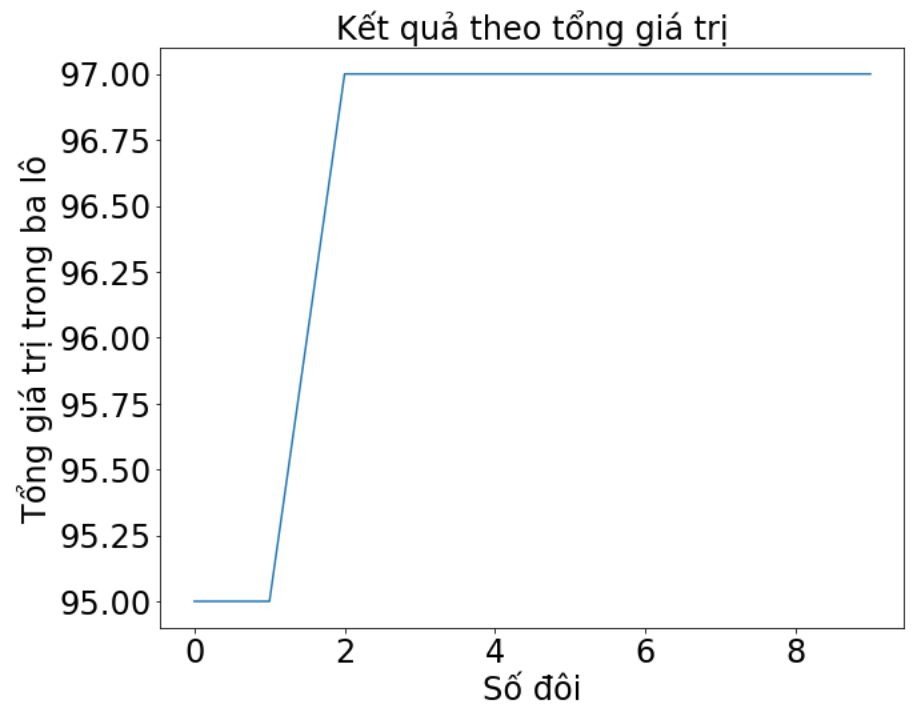
\includegraphics[width=8.5cm]{r1.png}
    \caption{Kết quả tổng giá trị tình huống 1}
    \label{fig:my_label}
\end{figure}

\item \textbf{Tình huống 2:} Các vật cho vào túi:  [1, 1, 1, 0, 0, 1, 1, 0, 0, 0, 1, 0] với khối lượng là 70 và giá tiền là 97.

\begin{figure}[!h]
    \centering
    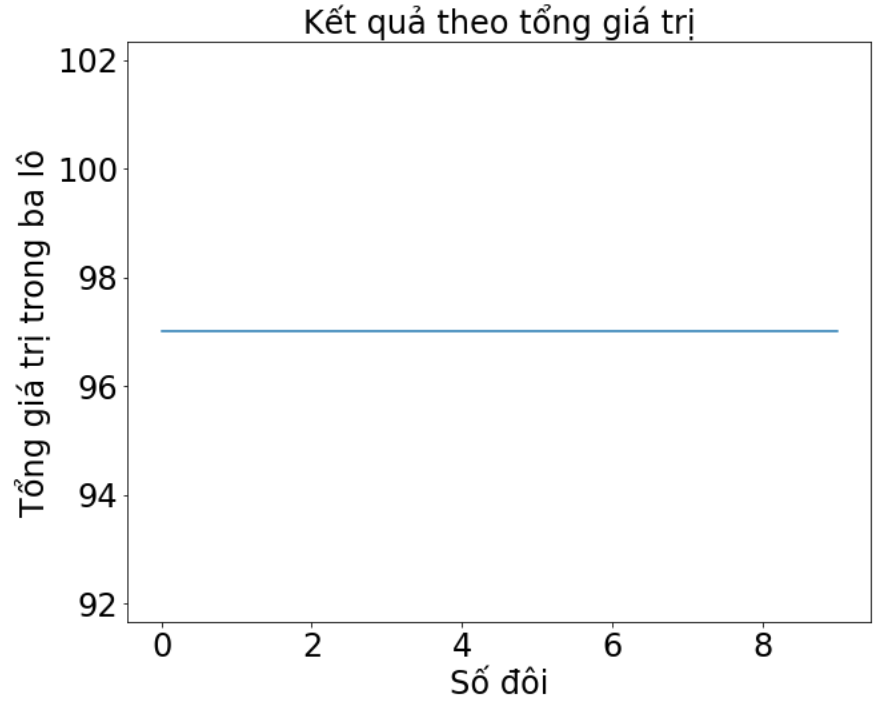
\includegraphics[width=8.5cm]{r2.png}
    \caption{Kết quả tổng giá trị tình huống 2}
    \label{fig:my_label}
\end{figure}

\item \textbf{Tình huống 3:}

Các vật cho vào túi:  [0, 0, 0, 0, 0, 0, 1, 1, 1, 0, 0, 0] với khối lượng là 70 và giá tiền là 101.

\begin{figure}[!h]
    \centering
    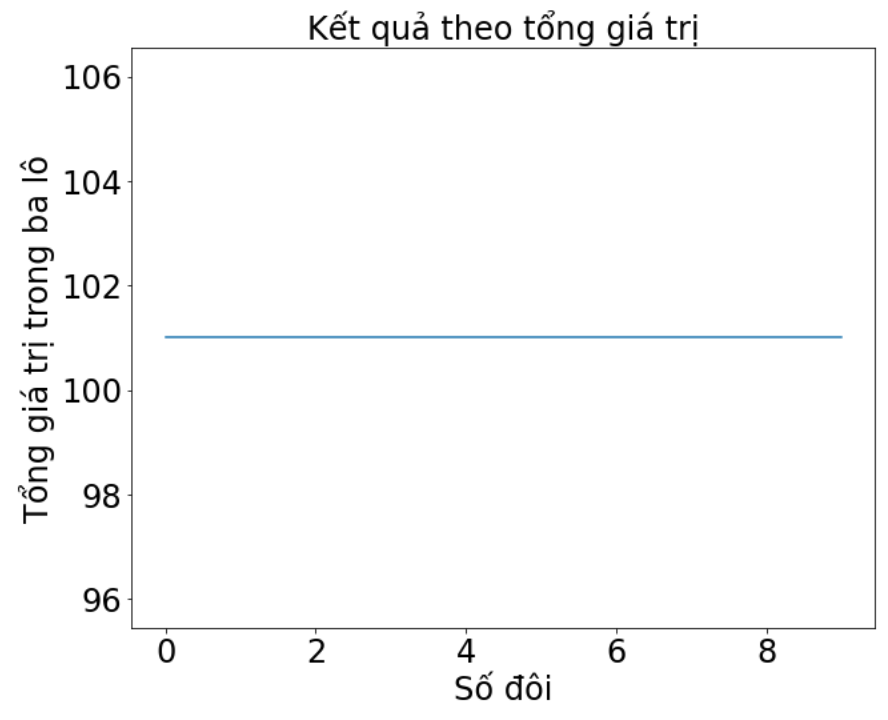
\includegraphics[width=8.5cm]{r3.png}
    \caption{Kết quả tổng giá trị tình huống 3}
    \label{fig:my_label}
\end{figure}

\pagebreak
\item \textbf{Tình huống 4:}

Các vật cho vào túi:  [0, 0, 0, 0, 0, 0, 1, 1, 1, 0, 0, 0] với khối lượng là 70 và giá tiền là 101.

\begin{figure}[!h]
    \centering
    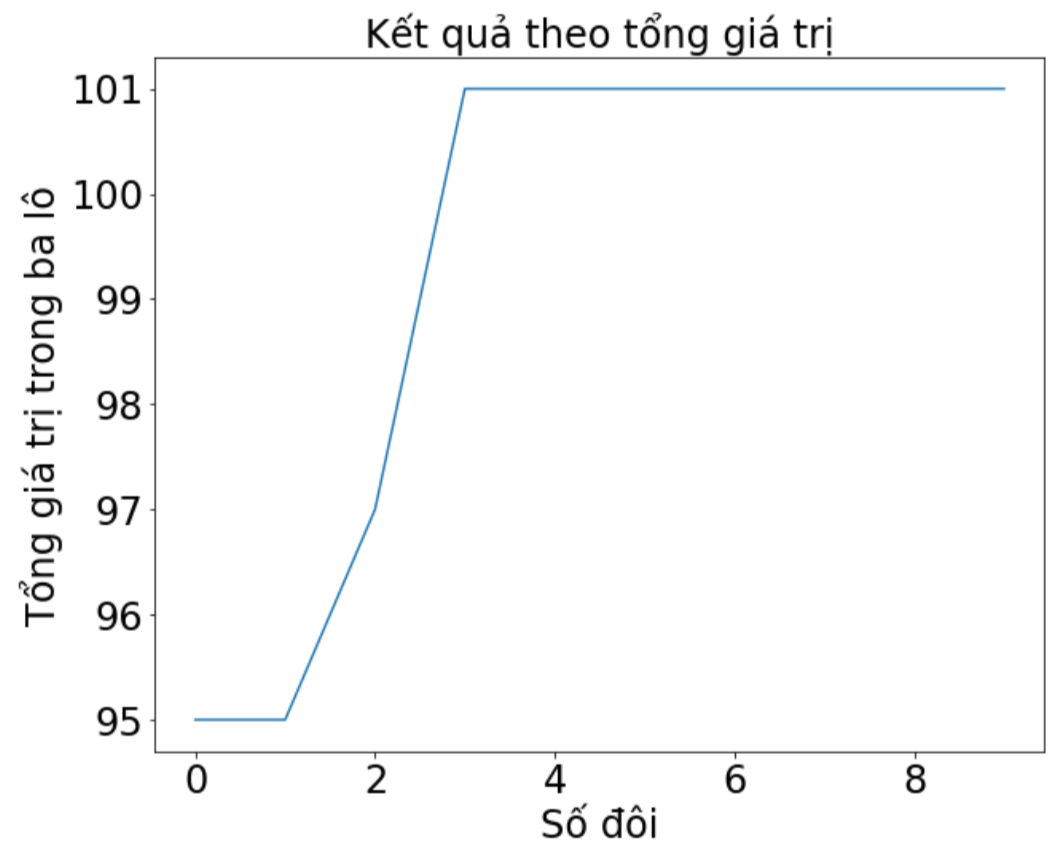
\includegraphics[width=8.5cm]{r4.png}
    \caption{Kết quả tổng giá trị tình huống 4}
    \label{fig:my_label}
\end{figure}

\end{itemize}

\textbf{Phân tích và đánh giá}

Với số lượng cá thể khởi tạo là 360 và 10 đôi, giải thuật di truyền trên bài toán Knapsack mang lại 4 trường hợp chính như sau:

\begin{itemize}[leftmargin=7pt]
    \item \textbf{Trường hợp 1:} Giá tiền là 97, tăng từ 95 ở lần thực hiện đầu tiên đến 97 đến số đôi thứ 2. 
    \item \textbf{Trường hợp 2:} Giá tiền là 97, đạt được ngay trong lần thực hiện đầu tiên.
    \item \textbf{Trường hợp 3:} Giá tiền là 101, đạt được ngay trong lần thực hiện đầu tiên. Đây là trường hợp thuật toán chạy tốt nhất.
    \item \textbf{Trường hợp 4:} Giá tiền là 101, đăng từ 96 ở lần thực hiện đầu tiên đến 101 đến số đôi thứ 2. 
\end{itemize}

\section{Giao diện người dùng}

Người dùng nhập vào số lượng các vật phẩm, giá trị và trọng lượng tương ứng và trọng lượng tối đa. Sau khi nhất nút "Run" thuật toán sẽ được thực thi và kết quả các vật phẩm được chọn, tổng giá trị và tổng số kí tương ứng sẽ được hiển thị lên màn hình.

\begin{figure}[!h]
    \centering
    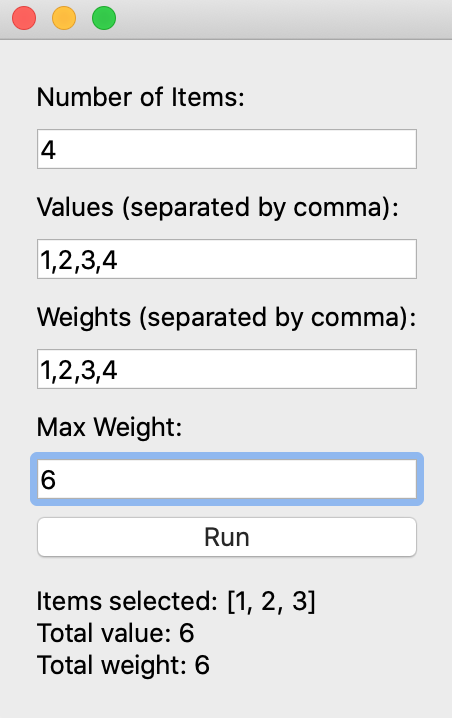
\includegraphics[width=6cm]{UI.png}
    \caption{Giao diện người dùng}
    \label{fig:my_label}
\end{figure}

Giao diện người dùng đơn giản cho phép người dùng nhập thông tin về một bài toán cái ba lô và chạy thuật toán di truyền để giải quyết vấn đề. Giao diện bao gồm một số trường nhập và một nút "Run", cũng như một nhãn để hiển thị Solution được tìm ra bởi thuật toán. 

\textbf{Mô tả giao diện:}

\begin{itemize}
\setlength\itemindent{-9pt}
\item
Trường nhập "Number of Items": Đây là một trường mà người dùng có thể nhập số lượng mặt hàng trong bài toán cái ba lô.

\item
Trường nhập "Values": Đây là một trường mà người dùng có thể nhập giá trị của các mặt hàng trong bài toán cái ba lô, được phân tách bằng dấu phẩy.

\item
Trường nhập "Weights": Đây là một trường mà người dùng có thể nhập khối lượng của các mặt hàng trong bài toán cái ba lô, được phân tách bằng dấu phẩy.

\item
Trường nhập "Max weight": Đây là một trường mà người dùng có thể nhập khối lượng tối đa mà cái ba lô có thể chứa.

\item
Nút "Run": Đây là một nút mà người dùng có thể nhấp để chạy thuật toán di truyền.

\item
Nhãn Solution: Đây là một nhãn nơi giải pháp cho bài toán cái ba lô sẽ được hiển thị sau khi thuật toán di truyền được chạy. Nó sẽ hiển thị các mặt hàng đã chọn, tổng giá trị của các mặt hàng đó và tổng khối lượng của các mặt hàng đó. 
\end{itemize}

\section{Kết luận}
\subsection{Các kết quả đạt được}

Thuật toán lần lượt cho ra giá trị các món đồ là 97 và 101. Trong đó, kết quả tối ưu nhất thuật toán mang lại là giá trị 101 trong lần thực hiện đầu tiên.

\subsection{Ứng dụng thực tiễn}

Giải thuật di truyền được sử dụng rộng rãi trong các lĩnh vực khác nhau để giải quyết các bài toán tối ưu hóa và tối ưu hóa đa mục tiêu. Trong đó, nổi bật là việc ứng dụng giải thuật di truyền trong ngành sản xuất và vận chuyển.

\textbf{Tối ưu hóa kế hoạch sản xuất} là một trong những ứng dụng thực tế của giải thuật di truyền. Trong quá trình sản xuất, các nhà máy cần tối ưu hóa các kế hoạch sản xuất để đảm bảo rằng sản phẩm được sản xuất với chất lượng tốt và trong khoảng thời gian ngắn nhất có thể, đồng thời đảm bảo sự tiết kiệm nguồn lực và chi phí.

Giải thuật di truyền được sử dụng để tìm ra kế hoạch sản xuất tối ưu bằng cách tạo ra một tập hợp các kế hoạch sản xuất khác nhau và tiến hóa chúng qua các thế hệ để tìm ra kế hoạch sản xuất tối ưu. Quá trình tiến hóa giúp tìm ra kế hoạch sản xuất tối ưu dựa trên các yêu cầu về nguồn lực, thời gian và chi phí.

Ví dụ, giải thuật di truyền có thể được sử dụng để tối ưu hóa kế hoạch sản xuất cho các sản phẩm như ô tô, máy tính, điện thoại di động, đồ gia dụng, và nhiều loại sản phẩm khác. Trong quá trình này, các thông số như số lượng sản phẩm cần sản xuất, số lượng máy móc và nhân công sẵn có được sử dụng để tạo ra các kế hoạch sản xuất khác nhau. Quá trình tiến hóa được sử dụng để tìm ra kế hoạch sản xuất tối ưu dựa trên các yêu cầu về nguồn lực, thời gian và chi phí.

Các ứng dụng của giải thuật di truyền trong tối ưu hóa kế hoạch sản xuất có thể giúp các nhà sản xuất tăng năng suất, giảm thời gian sản xuất, giảm chi phí sản xuất và nâng cao chất lượng sản phẩm.

\textbf{Tối ưu hoá đường vận chuyển} là một trong những ứng dụng phổ biến của giải thuật di truyền. Bài toán này được sử dụng để tìm kiếm lộ trình vận chuyển hàng hóa tối ưu từ các nhà máy đến các điểm bán hàng và kho hàng, nhằm giảm thiểu chi phí vận chuyển.

Các thông tin cơ bản cần có để giải quyết bài toán này bao gồm các điểm khách hàng và kho hàng cần vận chuyển hàng đến, số lượng hàng hóa cần vận chuyển, các ràng buộc về thời gian và chi phí vận chuyển giữa các điểm.

Giải thuật di truyền có thể được sử dụng để giải quyết bài toán này bằng cách sử dụng các cá thể trong quần thể để đại diện cho các lộ trình vận chuyển khác nhau. Mỗi cá thể được mã hóa thành một chuỗi gen, trong đó mỗi gen đại diện cho một điểm trong lộ trình vận chuyển. Quá trình lai ghép và đột biến được sử dụng để tạo ra các thế hệ mới của quần thể, nhằm tìm kiếm các lộ trình vận chuyển tối ưu hơn.

Để đánh giá độ tốt của một lộ trình vận chuyển, ta cần sử dụng hàm mục tiêu, thường là chi phí vận chuyển hoặc thời gian vận chuyển. Hàm mục tiêu này sẽ được áp dụng cho từng cá thể trong quần thể, và các cá thể tốt nhất sẽ được chọn để tiếp tục lai ghép và đột biến ở các thế hệ sau.

Thuật toán di truyền cũng có thể được sử dụng cho các nhiệm vụ cải thiện hình ảnh trong thị giác máy tính, chẳng hạn như cải thiện độ tương phản, làm mờ nhiễu và làm sắc nét hình ảnh [\cite{812529,6557714}]. Trong cải thiện độ tương phản, thuật toán di truyền có thể được sử dụng để tìm các tham số kéo giãn độ tương phản tối ưu cho một hình ảnh để cải thiện chất lượng hình ảnh. Trong làm mờ nhiễu, thuật toán di truyền có thể được sử dụng để tối ưu hóa các tham số của bộ lọc (kernel) và giảm nhiễu trong khi vẫn giữ được chi tiết hình ảnh. Trong làm sắc nét, thuật toán di truyền có thể được sử dụng để tối ưu hóa các tham số bộ lọc làm sắc nét để tăng cường cạnh và chi tiết của hình ảnh [\cite{bhandarkar1994edge}]. Những ứng dụng này của thuật toán di truyền trong việc cải thiện hình ảnh có thể dẫn đến cải thiện đáng kể về chất lượng hình ảnh và được sử dụng rộng rãi trong các lĩnh vực khác nhau như hình ảnh y học, đo lường từ xa và nhiếp ảnh số.

\subsection{Những hạn chế và hướng phát triển}

Giải thuật di truyền là một trong những phương pháp được sử dụng rộng rãi để giải quyết các vấn đề tối ưu trong nhiều lĩnh vực khác nhau. Tuy nhiên, giải thuật di truyền cũng có một số hạn chế cần được lưu ý. Một trong những hạn chế chính của giải thuật di truyền là khả năng rơi vào tối ưu cục bộ, khiến cho giải thuật không đảm bảo tìm được giải pháp tối ưu toàn cục. Ngoài ra, việc chọn tham số và xác định hàm mục tiêu cũng là những thách thức khó khăn trong quá trình sử dụng giải thuật di truyền. Để tăng khả năng tìm kiếm và cải thiện hiệu quả của giải thuật di truyền, các nghiên cứu hiện nay đang tập trung vào việc phát triển các chiến lược mới cho lai ghép và đột biến, kết hợp giải thuật di truyền với các phương pháp khác, và áp dụng các phương pháp tăng tốc tính toán để giảm thời gian tính toán và đáp ứng được nhu cầu sử dụng giải thuật trong các vấn đề có quy mô lớn.

\section{Phụ Lục}

Tất cả các mã nguồn cài đặt thuật toán và giao diện có tại \texttt{\url{https://github.com/quocviethere/GA-Knapsack}}

\pagebreak
\bibliographystyle{dinat}
\bibliography{citation}
\nocite{*}
\end{otherlanguage*}
\end{document}
